\chapter{An Approach for Reproducible Analysis}

\begin{center}
  \textit{If you're doing an experiment, you should report everything that 
    you think might make it invalid - not only what you think is right about it; 
    other causes that could possibly explain your results; and things you 
    thought of that you've eliminated by some other experiment, and how they 
    worked - to make sure the other fellow can tell they have been eliminated.}

 - Richard Feynman
\end{center}



NMR data analysis is irreproducible because insufficient information is
captured during the process.  A strategy is needed to facilitate 
reproducibility of the data analysis process.
This chapter will describe in more detail the common characteristics of
the missing data and what role they play as well as why it is important to
capture them, a model for capturing that data, and a strategy for using
the model during the analysis process.


\section{Current data models}
% TODO
... an outline of the BMRB and/or CCPN data models, as well as what they 
don't capture, and how that renders their use irreproducible ...

%  \item Problem: undeposited data (both primary and meta).  
%  Current depositions to the BMRB do not include extraneous 
%  results, intermediates, or deductive meta data.  

%  \item uncaptured primary and meta data: while contemporary NMR databases, 
%  such as the BMRB, archive, persist, and disseminate data and analysis 
%  results of completed structural, dynamics, and binding studies, the 
%  archived data and analysis do not include full information on GSSs 
%  and resonances, nor the meta data of manual analysis.  This is because the 
%  data is thrown away during the analysis process and not available for deposition.
% remember to blame this on tools and on current practices, and not on the BMRB



\section{Missing data and its role in analysis}
The key deficiencies causing irreproducibility are 
missing primary data (both extraneous results as well as intermediates), 
missing meta data relating to the deductive process of reasoning employed 
for manual analysis, and undeposited data (both primary and meta).  

% need to cover what the data is, how it plays a role in NMR analysis, 
% why it's important to capture
As was described in earlier sections, 
spectral analysis, including peak picking, GSS construction, GSS and resonance
typing, sequential GSS assignment, and sequence-specific GSS assignment is 
accomplished using a step-by-step process of deductive reasoning 
which is often augmented by computational tools.  The computational 
results may be subject to manual validation, correction, and extension
\cite{guerry2011automated}.  This section will explore the various types
of data involved.


\subsection{Deductive process of reasoning}
This data describes the 
deductive process of reasoning employed in manually interpreting a feature 
of the primary data.  It is important because it provides the explanation 
of why something was done.

As was covered earlier, the deductive process of reasoning which plays
a major role in data analysis generates intermediate data sets.  Associated
with the generation of these data sets is a rule employed for deduction.

% TODO do I need to say something about the proposed library of deductive reasons? or does that come later?
Each rule is an embodiment of NMR-specific knowledge of how to interpret a
data feature.  In general, a deductive rule requires an input, produces an
output, and has an intuitive justification for its action.  
% TODO example

Application of these rules provides a rationale for manual modifications.  The
rationale is a justification that the change modification is correct, as
well as an indication of why the change was made.  Therefore, capturing the
deductive rules employed enables verification of the veracity of modifications. 
It also facilitates knowledge transfer, both in the contexts of collaboration
and teaching, by providing a meaningful annotation (with reference to the
domain of NMR) for actions taken.

... a description of how manual analysis is related to deductive reasoning ...
Manual analysis follows a general pattern:
\begin{enumerate}
  \item identification: a feature of the data is identified as amenable to 
  interpretation.  For example, the feature may be a false negative (such as 
  a signal peak misclassified as noise by the automated peak-picker), a false 
  positive (such as an artifactual peak misclassified as signal), or an 
  ambiguity (such as overlapped GSSs, causing clustering algorithms to fail).
  \item pattern recognition: the spectroscopist identifies a potential method 
  for interpreting the feature based on his/her domain knowledge of NMR and 
  experience with interpretation of previous data sets.  For example, such 
  methods may take the form of deductive rules:  if <the data matches a 
  certain pattern>, then <it could be interpreted a certain way>. 
  See Figure-\ref{deduction}.
  \item application of the rule to the data feature.  The chosen rule is 
  applied, and the result of the interpretation is included back into the 
  data set.  The result may now be used to drive further deductions.
  \item repeat -- go to step 1 to identify features for further interpretations
This method is a form of iterative, sequential deduction.  The key components 
are the ordered series of steps, the state of the data before and after each 
step, and the deductive rules used to make interpretations at each step, as
 Figure-\ref{deductive_process} shows.  In 
addition, it should be noted that the final data set can not be regenerated 
using automated tools alone if there are any manual modifications made to 
tool output.
\end{enumerate}


\subsection{Deductive contexts: intermediate results}
The output of a 
computational tool, whether used for peak-picking, GSS construction, 
or sequence-specific GSS assignment, is often modified to correct 
mistakes.  This introduces a discrepancy between the output of the tool 
given the input and a suitable parameterization, and the final data set.  
By capturing a snapshot of the output of the tool immediately after it is 
run, and before modifications are made, this discrepancy is rectified.
Similarly, during manual analysis and modification of results, the state of 
the data is continually changing and determines which analyses may be made.  
For example, assignment of a GSS to a residue may allow a further 
unambiguous assignment of a different GSS to a residue (an assignment 
which previously would have been ambiguous) by eliminating one of two 
assignment possibilities based on matching amino acid type.  This shows that 
the state of the data determines what deductions can be made.  Therefore, it 
is important to capture these intermediate states before and after deductions.

An important feature of the analysis process is that the final results are
not the output of a single replicable step, but rather of a series of steps
of refinement and modification.  Thus, the analysis process implicitly 
generates a new data set (from the previous one) after every modification, 
whether manual or automated.

Implicit in the sequence of data sets are logical dependencies of derived
data upon features of the previous data set: the context of each deduction
is important, because the exact context determines what deductions may be
made and the confidence level of each deduction. % TODO an example

% TODO I need to discuss what the intermediate results need to do
%   i.e. they need to make the process recapitulatable
%   and this is done by capturing the contexts

The importance of capturing intermediates is due to the dependence of 
deductions on context: without knowing the context, it is impossible to 
evaluate the correctness, confidence, and alternative interpretations of
a deduction.  In standard approaches to analysis, the contexts are not
captured; they are implicit.  By making the contexts explicit, it becomes
possible not only to fully recapitulate the process of analysis, but also 
to employ error detection and correction strategies by analysis
of deductions and their contexts.  
An interesting side-effect of capturing
contexts is that analysis can be restarted in the middle, by selecting an
appropriate context and applying a different deduction.

% TODO
% come up with a simple example that demonstrates: 
%   1) the dependence of deductive ability on context
%   2) the concept and utility of multiple snapshots
%   3) the concept and utility of tracking logical dependencies


\subsection{Extraneous results}
Standard approaches use the 
assumption that all peaks are true signal, with no provision for storing peaks 
determined to be processing artifacts or noise.  Such spurious peaks are simply 
deleted and do not show up in the final results.  This is a problem because the 
fact that a peak was found, and later interpreted as noise does not show up in 
the final data set.  The same problem applies to GSSs that are found 
but can not be assigned to any residue of the sample of interest, or are 
believed to correspond to atoms of a contaminant.  Such GSSs should 
be represented in the final data set.

During analysis, some portion of the positive results are not of direct interest
to the final answer.  Not only peaks, but also resonances and GSSs are included.
The positive results include both false positives, caused by noise or
artifacts, and true positives, caused by contaminants.

Although not of direct interest, such extraneous results play a role in 
the process of analysis: as was covered earlier, when making a manual
modification, a deductive rule is applied to a context (data set).  Changing 
the context affects which rules apply and what deductions are made; 
therefore, as a part of the context, extraneous results matter during analysis. 
If incorrectly identified or left unrecognized, extraneous features can
lead to incorrect peak picking, chemical shift assignments, GSSs, and GSS
assignments.

A further benefit of capturing extraneous results is the ability to distinguish
between identifying a data feature and interpreting it.  In other words, peaks
picked during peak picking are treated as positives, this is the "identification"
phase; in the later "interpretation" phase, these peaks are separated into
false positives and true positives.  This allows rectification of the 
discrepancies between uncorrected computational results and the final,
deposited results as well as marking potentially suspicious results for 
future perusal.  It should also be noted that picking a peak, then
interpreting it as extraneous and discarding it is typically not reported in
final data sets, despite containing important information.
There is a balance between false positives and false negatives \cite{pine};
false negatives are more undesirable \cite{pine, saga, guntert2009automated},
and capturing extraneous results helps to avoid this tradeoff: by reducing
the cost of a false positive, tools are free to focus on avoiding false
negatives.

The process of separating positives into false and true is prone to 
introducing bias; by keeping and reporting the initial results, such bias
can be estimated.  This is not possible if the extraneous results are not
reported, and also allows the feature identification phase to proceed
without bias, since error correction will be applied at a later stage. 
By providing additional context, it may be possible to estimate the quality 
of an analysis, where errors may be most likely found in the borderline 
cases; it will also help assigning confidence levels to datums by not.
Additional quality measures enabled include the number of peaks found by the
peak-picker, the number of false positives, the number of peaks assigned to
GSSs, and the number of GSSs assigned to residues.  It may also be possible
to estimate contamination, incompleteness and overcompleteness, overfitting, 
and consistency.


\subsection{Incompletions, uncertainties, ambiguities: notes}
During the course of data analysis, it is often the case that odd, ambiguous,
abnormal, or otherwise unexpected situations noticed during analysis
\cite{nuseibeh2000inconsistency}.  
% TODO however, no record is made, blah blah .... these are valuable b/c blah blah
As notes indicate the deficiencies and 
potential problems present in a data set, they are valuable to future 
perusers as they highlight how a data set is flawed and how it can be improved.

Due to the difficulties inherent in data analysis, situations are reached
in which the interpretation of a specific feature is problematic:
\begin{itemize}
  \item uncertain or impossible.  The evidence for a particular deduction 
    is not solid.
  \item ambiguous.  Multiple interpretations of a feature are consistent
    with the data and satisfy the constraints.  It is not possible to choose
    between them.
  \item inconsistent.  The data set is in an inconsistent state, or a 
    deduction would leave it in an inconsistent state.
\end{itemize}
A simple example is non-stereospecific sidechain proton assignments: 
a residue such as a Histidine or Lysine which has two beta protons will 
often give rise to two resonances, one for each beta proton; however, 
without additional information, it is impossible to assign a resonance to
a specific atom.  A related example is caused by the two delta and epsilon
protons in Phenylalanine and Tyrosine aromatic sidechains; the two resonances,
even if distinguishable, can not be uniquely assigned to atoms.  In both
cases, the ambiguity is resolvable through the use of additional information;
however, before that additional information is provided, it is useful to be
able to store what is known -- that there are two peaks, each of which 
corresonds to one atom, but exactly which is unsure -- as an indication to
future analysis or perusal that a problem has been identified but not yet
solved.

The key idea is, given the inevitability of such problems during data
analysis, to create facilities for explicitly recognizing, discussing, 
and handling such problems \cite{robillard2007concerns}. 
Several strategies for such an approach 
are covered in \cite{nuseibeh2000inconsistency} including deferral of the
problem while flagging it for later follow-up.

Enabling the representation of such data has similarities to the probabilistic
approach applied by PINE \cite{pine} to great effect.  
PINE deals with the innate uncertainty of data 
analysis by resolving the tradeoff between false positives and false 
negatives through association of a probabilistic confidence metric with each
feature interpretation; low confidence values are used as evidence that an
interpretation is suspicious and needs additional verification or data.
In a complementary approach, capturing notes of analysis issues also 
resolves the tradeoff for manual analysis, by enabling the association of
an explanatory or warning message with suspected low-quality deductions.
In addition, the message may contain more information than a scalar: it may
necessarily refer to multiple conflicting pieces of the data set in the case
of a contradiction.

% TODO add a picture
Correctly identifying and characterizing peaks in the presence of significant
amounts of overlap is a notoriously difficult problem \cite{guerry2011automated}.
The number, position, and intensity of peaks become distorted by the overlap.
In such a case, it may not initially be possible to fully and correctly
resolve the overlap (although later information from additional spectra, such
as a higher-dimensional spectrum in which the additional dimension removes
the overlap, may resolve the problem); a note explaining that overlap is
suspected and that the characterizations may be in error points this out.

% TODO add a picture
Building unambiguous and complete sequential GSS assignments is complicated 
when multiple GSSs have the same or nearly the same chemical shift values
for resonances which are or potentially may be assigned to CA, CB, CO, or the
corresponding (i-1) atoms.  Leaving a note in the data set describing what
the ambiguity is ensures that this information is not lost, and is clearly
marked for re-analysis when more data becomes available.
% TODO make sure I don't describe the solution in this section -- rather, it should be about the problem !!


\section{A Model for Reproducible NMR}

\subsection{Data models}
A data model is a means of specifying the structure of information  
\cite{codd1970relational}.  This
information may be used as inputs and outputs for computational tools, or
it may be archived and available for reference use.  Data models are useful
because they provide a formal specification of the structure, which enables
unambiguous, correct, and automated use of data.  Data models are
abstract specifications; they must be implemented in source code in order
to become a usable artifact.

In the field of NMR, both the BMRB \cite{bmrb} and CCPN \cite{ccpn} have
created descriptive, extensive and useful data models, and have implemented them 
in programs and as Application Programming Interfaces (APIs).  These are used
by additional programs to help manage the exchange of data with external
programs.

This section will cover a data model for reproducibility.  Once a data
model exists, it can be implemented as part of a software program that
facilitates reproducible data analysis, as will be covered in a later 
chapter.  The core of this data model is formed by the BMRB \cite{bmrb}
and CCPN \cite{ccpn} data models.  These models are then extended with
several additional data types and properties in order to enable 
reproducibility.


\subsection{Deductive reasoning}
In a VCS, each snapshot is annotated with a commit message that describes 
the how and why of the snapshot -- what problems does it address, what 
features does it add.  Similarly, for capturing the data of the process of 
sequential deduction, the reasoning used describes the change to the data 
set and why it was made.  In order to support the capture of this meta data, 
an extensible library of commonly used deductive reasons enables the user to 
quickly and easily make deductions and describe the reasoning used.  These 
deductive reasons are then referenced in snapshot annotations.

A model for the deductive process of rule application to a data set to 
produce a modified, new data set requires components for both the rules 
themselves as well as the use of rules.  

A library of rules was built which enumerates deductive rules based on 
established practices during data analysis \cite{guerry2011automated, hncacb,
hnco, cbcaconh, hbhaconh, picky, xeasy, sparky, ccpn}.  For each rule, 
a meaningful name, an explanation of the rule's meaning, its intended use,
its intended result, and examples was collected.

During analysis, one or more rules are applied to make a deduction.  This
is capture in Figure-\ref{deduction_model}.

% TODO clean up library so that it's usable
% TODO present most or all of the library in picture and textual format

Here are several commonly used deductive reasons, the full list can be found
at \url{https://github.com/mattfenwick/PeakPicker/tree/master/library}:

\subsubsection{peak position}
Certain peak position can indicate whether a peak is signal, noise, or an 
artifact.  These positions include spectral regions that are expected to be 
empty, and projections of intensity along spectral edges.

\subsubsection{peak intensity}
Peaks from the same atom may have similar intensities. 
Signal, noise, and artifacts may have characteristic intensities.

\subsubsection{peak lineshape}
Peaks from the same atom may have similar lineshapes.
Signal, noise, and artifacts may have characteristic lineshapes.
 
\subsubsection{peak pattern}
Phase errors and truncations give rise to characteristic dispersive lineshapes
and sinc wiggles, respectively.  When using a naive peak picker, these may
be picked as a series of smaller peaks radiating out from a more intense,
central peak.

\subsubsection{sign of peak amplitude}
In some experiments, all true peaks are expected to have the same sign.  In
other experiments, such as the HNCACB, some peaks are expected to consistently
have a single sign, and another set of peaks are expected to consistently 
exhibit the opposite sign.

\subsubsection{chemical shift matching: assign peaks to GSS}
Based on matching of corresponding peak dimensions, peaks are combined into
GSSs.  The matching of peaks may be within a single spectrum, or between 
multiple spectra -- as long as the spectral dimensions match (both nucleus
and atomtype).  The tolerances allowed are important in determining which
peaks match.

\subsubsection{chemical shift matching: recognize noise and artifacts}
A potential signal peak may be recognized as noise or artifactual based on
missing of matching peaks in other or the same spectra that would be expected
if it were a true peak.

\subsubsection{chemical shift matching: peak}
One or more peaks assigned to a GSS may be used to peak a new peak missed by a
peak picker, based on matching one or more chemical shifts of the existing peaks
as well as spectral features.

\subsubsection{chemical shift matching: resonance to peak dimension}
The assignment of a peak dimension to a resonance can be used to assign another
peak dimension from the same GSS to the same resonance, if the chemical shifts
match.

\subsubsection{BMRB statistics: resonance typing}
The atomtype of resonances can often be assigned unambiguously using BMRB
statistics.  Process of elimination may also be employed.

\subsubsection{sidechain Tryptophan}
Sidechain Tryptophan GSSs exhibit a characteristic peak pattern with 
characteristic chemical shifts, which may be found in the BMRB.

\subsubsection{sidechain Asparagine/Glutamine}
Asparagine and Glutamine produce characteristic peak patterns in H-N-based 
experiments, due to their two sidechain protons.  These resonances consistently
appear in the same spectral region, making them easy to identify.

\subsubsection{sidechain Arginine}
Arginine sidechain GSSs resonate at characteristic chemical shifts, and may
even be subject to splitting if they appear sufficiently far outside of the
decoupling band.

\subsubsection{resolve overlap: peak to GSS}
When peaks overlap, it is difficult to assign them correctly to GSSs.  However,
the resonances may be resolvable in additional spectra, which then makes it
possible to return to the first spectrum and correctly resolve its overlap.

\subsubsection{peak sign and GSS type: resonance typing}
The GSS type and peak sign can be used in conjunction with certain pulse 
sequences to determine resonance types.  For example, in an HNCACB spectrum, 
the positive peak of a Glutamine sidechain is a CG and the negative is a CB 
(or vice versa).

\subsubsection{experiment and GSS type: resonance typing and GSS-peak}
This is similar to the previous reason.  
For example, hbCBcgcdHD experiment targets aromatics; a peak from that spectrum
that matches a GSS not typed as an aromatic, can not be assigned 
to that GSS.

\subsubsection{backbone Alanine}
Alanine's CB resonates at a characteristic chemical shift relative to other 
CB's due to its lack of additional Carbon atoms.

\subsubsection{backbone Gly}
Glycine's CA resonates at a characteristic chemical shift relative to other
CA's, and also lacks a CB atom.  In experiments such as an HNCACB or C(CO)NH-Tocsy,
Glycine strips appear without a CB peak.

\subsubsection{backbone Ser/Thr}
Serine's and Threonine's CB resonates at a characteristic chemical shift relative
to other CB's due to the -OH groups.

\subsubsection{chemical shift matching: GSS-GSS and resonance typing}
Matching Carbon strips from 3-dimensional experiments are used to build 
sequential GSS assignments and resolve some resonance types simultaneously. 
For example, given two HNCACB strips, chemical shift matching, and relative 
intensities, the sequential GSS assignments and CA(i)/CA(i-1) and CB(i)/CB(i-1) 
resonance typing assignments can be made, such that the following conditions
are satisfied (note that the last two are not inviolable):
\begin{itemize}
  \item i-1 peaks in following ss should be matched by i peaks in preceding ss
  \item intensity of HNCACB i-1 peaks should usually be less than intensity of i peaks in same ss
  \item intensity of HNCACB i-1 peaks should usually be less than intensity of matching i peaks in preceding ss
\end{itemize}

\subsubsection{unexpected peak: peak type}
A specific number of peaks are expected for a GSS in a given spectrum.
Extra peaks -- beyond the expected number -- may be artifacts or noise.

\subsubsection{GSS chain and primary sequence: GSS-residue}
A GSS chain can be assigned to residues based on the amino acid types of the 
residues and their match to the GSS typings.  It is not necessary that every
single GSS is unambiguously typed.
The process of elimination is useful in this deduction; for example, if the
GSS is an Arginine, and there's only one unassigned Arginine residue remaining,
the GSS may correspond to the Arginine.

\subsubsection{extend GSS-residue fragment}
A GSS chain already assigned to specific residues may be extended at the ends.
In addition to the constraints rules given in 
"chemical shift matching: GSS-GSS and resonance typing",
GSS typings must match the residue typing, or the BMRB statistics if untyped.

\subsubsection{BMRB statistics: resonance typing}
The BMRB average chemical shift stats -- along with the sstype assignment -- 
are useful for spectra such as the C(CO)NH-Tocsy, HBHA(CO)NH, and 
HC(CO)NH-Tocsy, where there are multiple peaks in a strip along a Carbon or
Hydrogen dimension. Most amino acid types feature good dispersion, making it 
easy to get the correct assignments straight directly from the statistics.

\subsubsection{Tocsy aliphatic sidechain: resonance typing}
After assigning HNCACB and HBHA(CO)NH spectra, C(CO)NH-Tocsy, HC(CO)NH-Tocsy 
and HCCH-Tocsy are used in conjunction:
the C(CO)NH-Tocsy peaks are used to find HCCH-Tocsy strips, which yields proton 
chemical shifts and match the HC(CO)NH-Tocsy peaks.  Also, each HCCH-Tocsy 
strip should have peaks in all the same 1H shifts.
BMRB statistics can be used to assign most peaktypes unambiguously.  
Splitting patterns also help to identify methylene groups.

\subsubsection{Tocsy peak pattern: resonance typing}
Several aliphatic C/H groups are difficult to distinguish using BMRB statistics,
including Leucine's CG, CD1, and CD2, as well as Isoleucine's CG2 and CD1, and
its QG2 and QD1. These can often be resolved by characteristic intensity 
patterns for each amino acid type due to the Tocsy nature of experiment,
as well as the observation that methyl peaks are often sharper and more intense.

\subsubsection{Cyana: stereospecific resonance typing}
Many pairs of atoms/groups give rise to two peaks which can not be immediately
assigned unambiguously, although it is known that each atom/group corresponds 
to one of the peaks, and the other atom/group to the other peak.
Examples include HB2/HB3 of Y, and QD1/QD2 of L.
For additional examples of ambiguities see \ref{stereospecific_ambiguities}.
Cyana can often resolve these ambiguities during structure calculation.


\subsection{Intermediate results}
The core of the strategy is based on that used by Version Control System (VCS) 
software tools \cite{vcs_concepts, hinsen2009vcs}, which are commonly 
applied for managing source code of 
software projects \cite{loeliger2012git, cvs, svn}.  
These tools were originally implemented in order to manage the change in 
source code over time, while retaining the ability to easily inspect past 
states of the code.  It was found that application of such tools led to 
large increases in productivity, robustness, correctness, and reduced 
faults \cite{fischer2003vcs}.  The core of a VCS is a model for change in data 
over time by storing multiple versions.  Versions are snapshotted, 
descended from previous snapshots, and annotated with a commit message 
which describes the what and the why of the change.  Similarly, in NMR 
during the process of sequential deduction, intermediate states form a 
chain.  By capturing these intermediates, similar advantages are gained 
(as in VCS).  While taking multiple snapshots of a large data set may 
seem wasteful of storage space, it is important to note that there are 
several approaches for compressing the snapshots to eliminate duplication; 
this essentially reduces the wasted space to zero.


% TODO needs some expansion and clarification of how this is novel
The strategy for modelling intermediate results is based on the data models
of existing version control systems, including Git \cite{loeliger2012git},
SVN \cite{svn}, and CVS \cite{cvs}.  The general outline of the solution 
is a sequence of snapshots of the data set, taken at carefully chosen 
moments during analysis, which show the full process of analysis by capturing
all changes.  Each snapshot -- other than the first -- contains a link to
the previous snapshot, as well as a set of data differences.  The differences
between snapshots provide the key value of this solution: they explicitly
show how the data set is changed over time.
Associated with each snapshot is a small amount of meta data to help describe
the snapshot, including a timestamp, author information, and a deductive
annotation, which describes the "why" of the changes and will be covered in
the next section.

% note that while the basic idea is taken from VCSs, the actual appropriate
%   use is going to be more heavily dependent on the domain of NMR
While the general solution is adapted from version control software, in order
to effectively capture intermediate NMR data sets, such that the process of
analysis is clear and understandable, the solution must be augmented to fit
the specific needs of the NMR domain.
In other words, capturing meaningful intermediate snapshots is challenging; it 
is not sufficient to capture them indiscriminately.  If snapshots are captured 
too infrequently, the situtation is not significantly different from current 
practices: the analysis process will not be reproducible.  If too many snapshots
are captured, reconstructing the logical dependencies will not be possible;
in addition, the valuable information may be difficult to identify compared to
the large amounts of useless information.  A third potential problem is 
collecting snapshots indiscriminately -- i.e. not in a manner that corresponds
to the actual process employed.  This, too, prevents later use of the 
intermediate data because the process has not been correctly captured.

Therefore, there are several principles of intermediate data collection which
must be observed in order to create a useful data set.  These principles help
to ensure that snapshots are created neither too often nor too rarely, and
that they are useful for future perusal:
\begin{itemize}
  \item time.
    Snapshots should be taken often enough that all modifications are captured.
    For example, when peaks are initially picked by an automated tool, and then 
    modified (perhaps sorting them into signal, noise, and artifact classifications)
    by manual adjustment, a snapshot must be taken immediately after the automated
    peak picker is run, and before any modifications are made.  When additional
    modifications are made, it is again necessary to take another snapshot before
    these changes, in order to capture the previous state of the data set -- which
    is otherwise lost if this is not done.
  \item content.
    Each snapshot should have a clear and simple focus on analyzing a single
    feature or performing a single type of interpretation.  For example, a snapshot
    should not include changes both to resonance typing and to peak lists if those
    changes are not inter-dependent.  % this ensure that logical dependencies are recoverable ? ... 
  \item cohesion.
    Similarly to the previous point, changes which are inter-dependent belong in
    the same snapshot.  For example, when assigning GSSs sequentially, assume there
    are two potentially matching GSSs based on CA and CB resonances, which however
    have not been specifically assigned i/i-1.  If one GSS is determined to be the
    first, and the other the second, then the CA(i), CA(i-1), CB(i), and CB(i-1)
    assignments of the resonances in both spin systems are determined.  These 
    changes all naturally belong in a single snapshot, since they are logically 
    co-dependent.
  \item logical dependencies must be recoverable.
    The previous two points enable recovery of deductive, logical dependencies.  
    The sequential process of deduction is the core of manual analysis, and 
    therefore it is important to capture it clearly.  This means that the 
    dependencies must be reconstructable from the sequence of intermediate data 
    sets.
\end{itemize}

% devote more space to discussing diffs/comparisons, logical dependencies
%   what, why, and how.  
%   also, how the VCS-based solution supports these goals
The primary goal of capturing intermediate data sets is to 
facilitate reproducibility by modeling and saving the process of analysis.  
A system which does so by capturing a sequence of snapshots of the data set 
at intermediate timepoints meets the requirements for reproducibility.
First, such a system is able to correctly recapitulate the changes over time
due to manual and automated analysis.  For example,
if an automated peak picker were used on a spectrum, and then the results
manually verified and corrected, if snapshots were taken at the appropriate
moments, the sequence of snapshots would show both the complete results of
the automated tool, as well as every manual change made.
% TODO should I say more here?
Second, by capturing the full context of each modification, the logical and 
temporal dependencies between various features of the data set are trackable.
% TODO what? the following doesn't make much sense
Additionally, capturing multiple intermediates allows rich comparisons to be made 
between snapshots.  These comparisons, combined with the deductive annotations,
indicate the changes made with each specific deductive reason. 


\subsection{Extraneous results}
Our approach is to allow any number of peaks and GSSs, and to 
augment them with additional data fields which distinguish between signal, 
noise, contaminants, etc.  This allows one to make a critical distinction 
between: 1) finding/recording a peak based purely on characteristics of 
the spectrum such as volume, height, relative height compared to noise, 
lineshape, and linewidth, and 2) interpreting a peak as signal, noise, 
etc. (and the same for GSSs).  Even peaks and GSSs for 
which no analysis is made can be kept in the data set without encumbering 
assignment of true peaks and GSSs.

To model extraneous results, the BMRB and CCPN models \cite{bmrb, ccpn}
were extended to support additional fields which distinguished between 
extraneous and primary data.
This applies to peaks, resonances, and GSSs.
The general approach for using this model is to never directly delete
a peak, resonance, or GSS, but rather to mark it as extraneous by modifying
its associated category from 'signal' to 'artifact', 'noise', 'contaminant'
etc.

For example, while using an interactive spectral analysis such as Sparky or
CCPN Analysis \cite{sparky, ccpn} for peak picking a spectrum, it is common
to run the automated, built-in peak picker and then to manually correct the
results by deleting some peaks and adding new ones.  This approach would
work differently; peaks would not be deleted.  If the category of each of the
peaks initially picked by the automated tool were 'signal', then the task of
the user would be to correct all of the categories for peaks which were 
determined to be signal or noise; note that these peaks would not be deleted
from the list.  They would remain in the list but with a different category
tag that would differentiate them from signal peaks.

A further category of extraneous data is peaks from amino acid sidechains; 
it is presented in Tables \ref{nhsqc_peaktypes}, \ref{hnco_peaktypes}, 
\ref{hncacb_peaktypes}, \ref{hbhaconh_peaktypes}, \ref{cconh_peaktypes}, and
\ref{hcconh_peaktypes}.  While most of the
peaks in these experiments correspond to backbone covalently bond atom groups, 
and are used for backbone sequential assignments, many sidechain GSSs are
visible as well.  Although these peaks are often ignored, they do contain
useful information.  They also can confound analysis if they are not properly
recognized as sidechain peaks.  Lastly, their presence is surprising to 
newcomers to the analysis process, as they are typically not explicitly 
recognized as part of the standard experiments.

% TODO a pictoral representation of this model
% TODO examples
% TODO 
% CCPN peak pick as initial peak list, then corrections I made as peak list 
% where each peak has additional fields


\subsection{Notes}
To model notes, the BMRB and CCPN models \cite{bmrb, ccpn} were extended
to support an additional data type: a note.  A note can refer to one or more
other feature of the data set, and also includes a textual description of
the nature of the problem, as well as an indication of how the problem might
be resolved (although that is optional).  As the purpose of a note is to
explicitly indicate known deficiencies, incompletions, or uncertainties in 
the data set, wherever and whatever they may be, this approach is able to do
so.
% TODO a pictoral representation of this model
% TODO example: odd feature in data, unable to resolve


\section{An implementation of the model}
% TODO a Sparky extension
... under construction ...


\section{Applying reproducible analysis: using the model}
This section presents some general advice for how to use the reproducibility
model effectively in practice.  It provides tips and suggestions, as well
as covering common problems and how they can be avoided.

\begin{itemize}
  \item one snapshot, one focus.  Keeping each snapshot focused on dealing
    with a single issue helps the process of analysis to remain understandable
    to later perusers.  This is because it makes the logical dependencies 
    more obvious; when a single snapshot contains many unrelated things, or
    is extensive enough that part of the snapshot depends on other parts, then
    it is no longer clear what the logical relationships are.  Keeping snapshots
    small and focused alleviates this issue.
  \item level of detail.  It is not necessary to exhaustively annotate every
    last single change; clearly, such an approach would be problematic because
    it would require far too much time and effort on the part of its users.
    Rather, the value of this reproducible approach is to clearly indicate 
    major issues and modifications.  The more important and the more time and
    brain power went into making a deduction, the more annotation it typically
    deserves -- in other words, a complicated deduction requires a complicated
    justification.  On the other hand, if multiple peaks are quickly and
    straightforwardly identified as artifactual with a minimum of effort, 
    only a bare minimum of annotation is needed; the deduction does not become
    clearer with additional annotation.
  \item apply the correct rule(s).
  \item record uncertainty and resolution.  When in doubt or difficulty 
    during analysis, record all information pertaining to the issues, whether
    as a note or extraneous data.  Even if the problem is easily or quickly
    solved, describing it creates a record of that problem which is valuable
    for later perusal.  Trends over such a record help to indicate more 
    large-scale problems, as well as illuminating troublesome spots for
    collaborators and learners.
\end{itemize}
   
% maybe talk about the culture of the lab notebook?
% could this belong in its own chapter?
% or in the software chapter, or in the 'reproducible data sets' chapter?


\section{Archiving reproducible data sets}
A major portion of the value derived from collecting reproducible data sets
is disseminating them so that others may obtain and use or inspect the data
in some way.  The standard means for sharing NMR-derived data is the BMRB
\cite{bmrb}, which uses the NMR-Star file format.  In order to enable archival
of reproducible data sets, we have collaborated with the BMRB to extend the
NMR-Star data dictionary, so that reproducible data sets may be collected and
deposited in the NMR-Star format.

The NMR-Star data dictionary, which may be found at 
\url{http://www.bmrb.wisc.edu/dictionary/}, catalogs the names, structure,
intended use, and definitions of the data types handled by the BMRB.


\section{Discussion}
By collecting reproducible data sets, the true information content used in
NMR spectroscopy is made explicit and visible.  This is analogous to how lab
notebooks are intended to be used in wet-lab work: as a means of recording
the crucial details describing how an experiment was done, so that the procedure
can be shared with and improved upon by others.  A key difference, however, is
that while lab notebooks have been in use for several centuries, the culture
of reproducibility of digital analysis is still in its infancy: we do not yet
have much experience with the what, how, and why of reproducibility in 
electronic media.

% TODO this is a pretty weak paragraph
The first key step, which I have described in this chapter, is to define what
the problems are -- in the form lost data -- and a model for what that data is.
Then the model must be applied in practice, and its correct use taught.

By extending standard existing models, the barrier to entry is greatly reduced,
and instead of requiring an abrupt and drastic change in the workflows of those
already using the standard models \cite{bmrb, ccpn}, the change to reproducible
analysis can be incremental and gradual.  This should help adoption.

Not only will such data sets make the process explicit, they will also help
make biases explicit.  It is possible that different research groups and
different analysis techniques have different innate biases; it is quite likely
that such biases will become obvious through the collection of these full data
sets.  Each bias will represent an opportunity for learning and for improving
the quality of analysis.


\clearpage
\section{Tables}

\begin{table}[h]
  \begin{tabular}{ | c | c | }
    \hline
    Covalently-bound atom group  &  Amino acid sequence  \\  \hline
    H-N                          &  [\^{}P]              \\  \hline
    HE-NE                        &  R                    \\  \hline
    HD21-ND2                     &  N                    \\  \hline
    HD22-ND2                     &  N                    \\  \hline
    HE21-NE2                     &  Q                    \\  \hline
    HE22-NE2                     &  Q                    \\  \hline
    HE1-NE1                      &  W                    \\  \hline
  \end{tabular}
  \caption{The covalent atom groups visible in the NHSQC experiment.}
  \label{nhsqc_peaktypes}
\end{table}

\begin{table}
  \begin{tabular}{ | c | c | }
    \hline
    Covalently-bound atom group  &  Amino acid sequence  \\  \hline
    H-N-C(i-1)                   &  .[\^{}P]             \\  \hline
    HE-NE-CZ                     &  R                    \\  \hline
    HD21-ND2-CG                  &  N                    \\  \hline
    HD22-ND2-CG                  &  N                    \\  \hline
    HE21-NE2-CD                  &  Q                    \\  \hline
    HE22-NE2-CD                  &  Q                    \\  \hline
    HE1-NE1-???                  &  W                    \\  \hline  % TODO the ???'s
  \end{tabular}
  \caption{The covalent atom groups visible in the HNCO experiment.}
  \label{hnco_peaktypes}
\end{table}
    
\begin{table}
  \begin{tabular}{ | c | c | }
    \hline
    Covalently-bound atom group  &  Amino acid sequence  \\  \hline
    H-N-CA                       &  .[\^{}P]             \\  \hline
    H-N-CA(i-1)                  &  .[\^{}P]             \\  \hline
    H-N-CB                       &  .[\^{}PG]            \\  \hline
    H-N-CB(i-1)                  &  [\^{}G][\^{}P]       \\  \hline
    HE-NE-CD                     &  R                    \\  \hline
    HD21-ND2-CB                  &  N                    \\  \hline
    HD21-ND2-CA                  &  N                    \\  \hline
    HD22-ND2-CB                  &  N                    \\  \hline
    HD22-ND2-CA                  &  N                    \\  \hline
    HE21-NE2-CG                  &  Q                    \\  \hline
    HE21-NE2-CB                  &  Q                    \\  \hline
    HE22-NE2-CG                  &  Q                    \\  \hline
    HE22-NE2-CB                  &  Q                    \\  \hline
  \end{tabular}
  \caption{The covalent atom groups visible in the HNCACB experiment.}
  \label{hncacb_peaktypes}
\end{table}

\begin{table}
  \begin{tabular}{ | c | c | }
    \hline
    Covalently-bound atom group  &  Amino acid sequence         \\  \hline
    H-N-HA(i-1)                  &  [\^{}G][\^{}P]              \\  \hline
    H-N-HA2(i-1)                 &  G[\^{}P]                    \\  \hline
    H-N-HA3(i-1)                 &  G[\^{}P]                    \\  \hline
    H-N-HB(i-1)                  &  [ITV][\^{}P]                \\  \hline
    H-N-QB(i-1)                  &  A[\^{}P]                    \\  \hline
    H-N-HB2(i-1)                 &  [PRNDCQEHLKMFSWY][\^{}P]    \\  \hline
    H-N-HB3(i-1)                 &  [PRNDCQEHLKMFSWY][\^{}P]    \\  \hline
  \end{tabular}
  \caption{The covalent atom groups visible in the HBHA(CO)NH experiment.}
  \label{hbhaconh_peaktypes}
\end{table}

\begin{table}
  \begin{tabular}{ | c | c | }
    \hline
    Covalently-bound atom group     &  Amino acid sequence  \\  \hline
    H-N-C*(i-1), * in (A)           &  G[\^{}P]             \\  \hline
    H-N-C*(i-1), * in (A, B)        &  [HDSNCAFYW][\^{}P]   \\  \hline
    H-N-C*(i-1), * in (A, B, G)     &  [EQM][\^{}P]         \\  \hline
    H-N-C*(i-1), * in (A, B, G2)    &  T[\^{}P]             \\  \hline
    H-N-C*(i-1), * in (A, B, G, D)  &  [RP][\^{}P]          \\  \hline
    H-N-C*(i-1), * in (A, B, G1, G2)    &  V[\^{}P]         \\  \hline
    H-N-C*(i-1), * in (A, B, G, D, E)   &  K[\^{}P]         \\  \hline
    H-N-C*(i-1), * in (A, B, G1, G2, D1)&  I[\^{}P]         \\  \hline
    H-N-C*(i-1), * in (A, B, G, D1, D2) &  L[\^{}P]         \\  \hline
    % sidechain 
    HD21-ND2-C*, * in (B, A)    &  N (sidechain)            \\  \hline
    HD22-ND2-C*, * in (B, A)    &  N (sidechain)            \\  \hline
    HE21-NE2-C*, * in (G, B, A)  &  Q (sidechain)           \\  \hline
    HE22-NE2-C*, * in (G, B, A)  &  Q (sidechain)           \\  \hline
    % TODO what about K, R, W sidechains?
  \end{tabular}
  \caption{The covalent atom groups visible in the C(CO)NH-Tocsy experiment.}
  \label{cconh_peaktypes}
\end{table}

\begin{table}
  \begin{tabular}{ | c | c | }
    \hline
    H-N-*(i-1), * in (HA2, HA3)                         &  G[\^{}P]             \\  \hline
    H-N-*(i-1), * in (HA, HB2, HB3)                     &  [HDSNCFYW][\^{}P]    \\  \hline
    H-N-*(i-1), * in (HA, QB)                           &  A[\^{}P]             \\  \hline
    H-N-*(i-1), * in (HA, HB, QG2)                      &  T[\^{}P]             \\  \hline
    H-N-*(i-1), * in (HA, HB2, HB3, HG2, HG3)           &  [EQM][\^{}P]         \\  \hline
    H-N-*(i-1), * in (HA, HB2, HB3, HG2, HG3, HD2, HD3) &  [RP][\^{}P]          \\  \hline
    H-N-*(i-1), * in (HA, HB, QG1, QG2)                 &  V[\^{}P]             \\  \hline
    H-N-*(i-1), * in (HA, HB2, HB3, HG3, HG3, HD2, HD3, HE2, HE3)   &  K[\^{}P] \\  \hline
    H-N-*(i-1), * in (HA, HB, HG12, HG13, QG2, QD1)     &  I[\^{}P]             \\  \hline
    H-N-*(i-1), * in (HA, HB2, HB3, HG, QD1, QD2)       &  L[\^{}P]             \\  \hline
    % sidechain
    HD21-ND2-*, * in (HB3, HB2, HA)   &  N (sidechain)                  \\  \hline
    HD22-ND2-*, * in (HB3, HB2, HA)   &  N (sidechain)                  \\  \hline
    HE21-NE2-*, * in (HG3, HG2, HB3, HB2, HA)   &  Q (sidechain)        \\  \hline
    HE22-NE2-*, * in (HG3, HG2, HB3, HB2, HA)   &  Q (sidechain)        \\  \hline
  \end{tabular}
  \caption{The covalent atom groups visible in the HC(CO)NH-Tocsy experiment.}
  \label{hcconh_peaktypes}
\end{table}

% TODO hcch-tocsy peaktypes

\begin{table}
  \begin{tabular}{ | c | c | c |}
    \hline
    Ambiguity type    &  Atoms        &  Amino acid types     \\  \hline 
    3 atoms, 1 peak   &  QB           &  A                    \\  \hline 
    3 atoms, 1 peak   &  QG1          &  I                    \\  \hline 
    3 atoms, 1 peak   &  QG2          &  [TI]                 \\  \hline 
    3 atoms, 1 peak   &  QE           &  M                    \\  \hline 
    2 atoms, 2 peaks  &  HA2/HA3      &  G                    \\  \hline 
    2 atoms, 2 peaks  &  HB2/HB3      &  [RHKDESNQCPLMFYW]    \\  \hline 
    2 atoms, 2 peaks  &  HG2/HG3      &  [RKEQPM]             \\  \hline 
    2 atoms, 2 peaks  &  HG12/HG13    &  I                    \\  \hline 
    2 atoms, 2 peaks  &  HD2/HD3      &  [RKP]                \\  \hline 
    2 atoms, 2 peaks  &  HD21/HD22    &  N                    \\  \hline 
    2 atoms, 2 peaks  &  HE2/HE3      &  K                    \\  \hline 
    2 atoms, 2 peaks  &  HE21/HE22    &  Q                    \\  \hline 
    2 atoms, 2 peaks  &  CG1/CG2      &  V                    \\  \hline 
    2 atoms, 2 peaks  &  CD1/CD2      &  L                    \\  \hline 
    2 atoms, 2 peaks or 2 atoms, 1 peak  &  HD1/HD2  &  [YF]  \\  \hline 
    2 atoms, 2 peaks or 2 atoms, 1 peak  &  HE1/HE2  &  [YF]  \\  \hline 
    2 groups of 3 atoms, 2 peaks  &  QG1/QG2  &  V            \\  \hline
    2 groups of 3 atoms, 2 peaks  &  QD1/QD2  &  L            \\  \hline
  \end{tabular}
  \caption{Ambiguities in stereospecific assignments}
  \label{stereospecific_ambiguities}
\end{table}


% figures
\clearpage
\section{Figures}

\begin{figure}[h]
  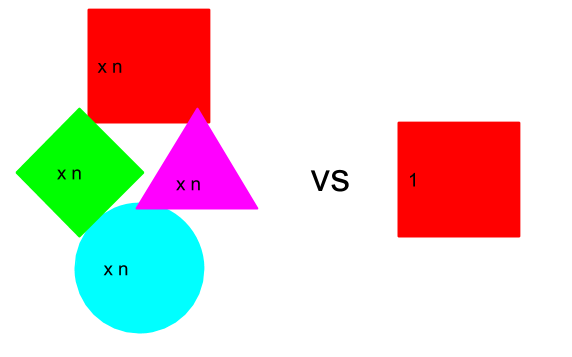
\includegraphics[scale=0.6]{figures/data_captured}
  \caption{A subset of generated data is captured}
  \label{data_captured}
\end{figure}

\begin{figure}
  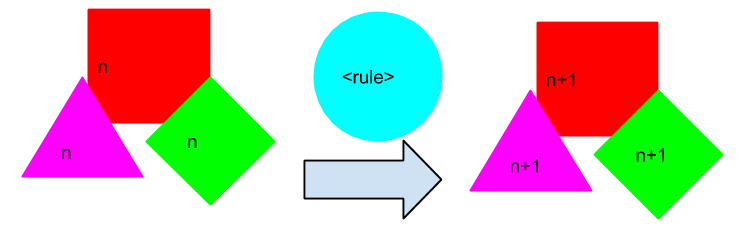
\includegraphics[scale=0.5]{figures/deduction}
  \caption{Applying a deductive rule to a data set is a deduction}
  \label{deduction}
\end{figure}

\begin{figure}
  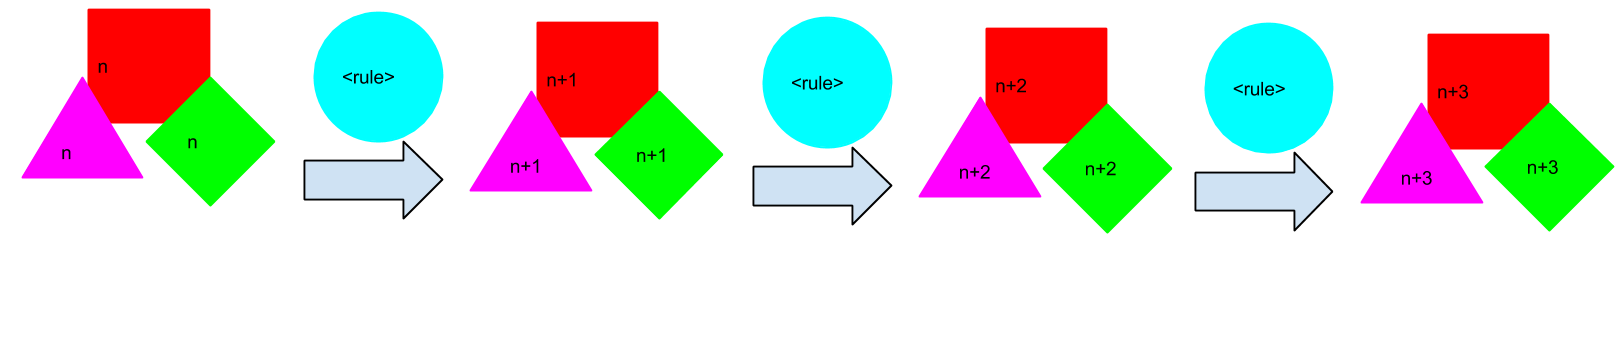
\includegraphics[scale=0.25]{figures/deductive_process}
  \caption{The complete manual analysis process is a series of deductions}
  \label{deductive_process}
\end{figure}

\begin{figure}
  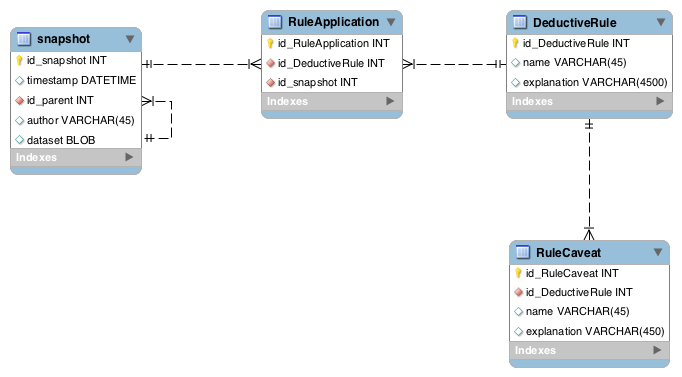
\includegraphics[scale=0.5]{figures/deduction_model}
  \caption{A relational model of a snapshot and deductions.}
  \label{deduction_model}
\end{figure}

